\documentclass[border=4pt]{standalone}
\usepackage{tikz}
\usepackage{pgfplots}
\pgfplotsset{compat=1.18}
\usetikzlibrary{shapes.geometric,arrows.meta,positioning,calc,fit,decorations.pathreplacing,backgrounds}
\definecolor{boxblue}{RGB}{225,238,252}
\definecolor{boxgreen}{RGB}{225,247,231}
\definecolor{boxorange}{RGB}{253,236,216}
\definecolor{boxgray}{RGB}{237,237,237}
\definecolor{boxred}{RGB}{253,226,226}
\begin{document}
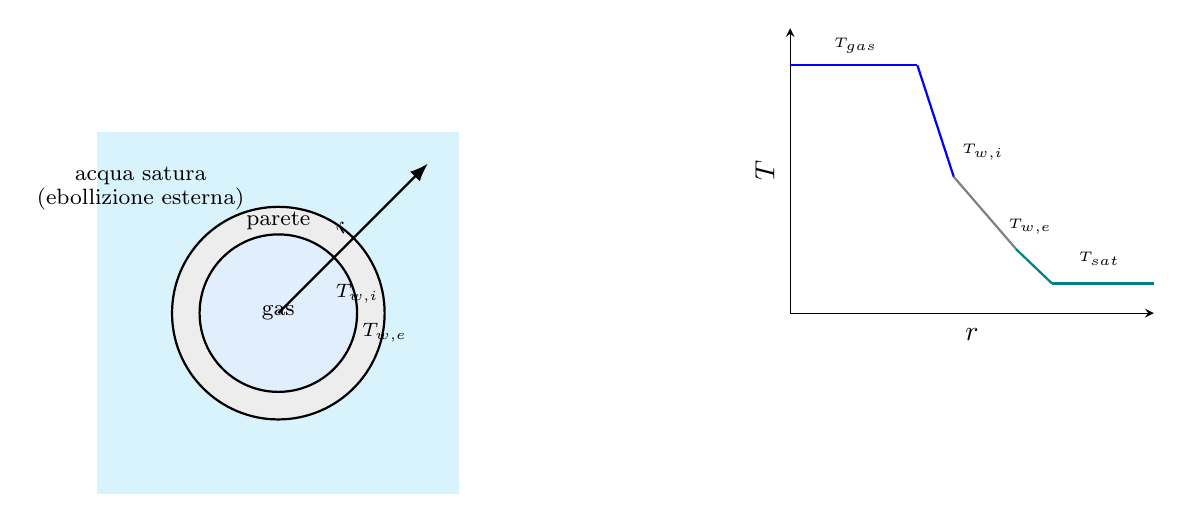
\begin{tikzpicture}
% Cross-section schematic
\begin{scope}
\fill[boxblue] (0,0) circle (1.0);
\fill[boxgray] (0,0) circle (1.35) circle (1.0);
\draw[thick] (0,0) circle (1.0);
\draw[thick] (0,0) circle (1.35);
\fill[cyan!15] (-2.3,-2.3) rectangle (2.3,2.3);
\fill[boxgray] (0,0) circle (1.35);
\fill[boxblue] (0,0) circle (1.0);
\draw[thick] (0,0) circle (1.0);
\draw[thick] (0,0) circle (1.35);
\node[font=\footnotesize] at (0,0) {gas};
\node[font=\footnotesize] at (0,1.17) {parete};
\node[font=\footnotesize] at (-1.75,1.75) {acqua satura};
\node[font=\footnotesize] at (-1.75,1.45) {(ebollizione esterna)};
\draw[-{Latex},thick] (0,0) -- (1.9,1.9) node[midway,above,sloped,font=\footnotesize]{$r$};
\node[font=\scriptsize] at (1.0,0.25) {$T_{w,i}$};
\node[font=\scriptsize] at (1.35,-0.25) {$T_{w,e}$};
\end{scope}
\begin{scope}[xshift=6.5cm]
\begin{axis}[
  width=6.2cm, height=5.2cm,
  xlabel={$r$}, ylabel={$T$},
  xtick=\empty, ytick=\empty,
  axis lines=left,
  ymin=0, ymax=1.15, xmin=0, xmax=1,
]
\addplot[thick,blue,domain=0:0.35,samples=2]{1.0};
\addplot[thick,blue,domain=0.35:0.45,samples=2]{1.0-(x-0.35)*4.5};
\addplot[thick,gray,domain=0.45:0.62,samples=2]{0.55-(x-0.45)*1.7};
\addplot[thick,teal,domain=0.62:0.72,samples=2]{0.26-(x-0.62)*1.4};
\addplot[thick,teal,domain=0.72:1.0,samples=2]{0.12};
\node[font=\tiny] at (axis cs:0.18,1.08) {$T_{gas}$};
\node[font=\tiny] at (axis cs:0.53,0.65) {$T_{w,i}$};
\node[font=\tiny] at (axis cs:0.66,0.35) {$T_{w,e}$};
\node[font=\tiny] at (axis cs:0.85,0.22) {$T_{sat}$};
\end{axis}
\end{scope}
\end{tikzpicture}
\end{document}
